\section{User Study 1}

% \begin{enumerate}
% \item Process of gameplay
% \item User's feedback for existing games
% \item User's imagination
% \end{enumerate}

In order to realize the current game play experience on google glass. We use games currently existing on google glass to perform our user study. Furthermore, with a view to understanding the response and feedback for different control style and game content from users, we choose four games, ``Balance'', ``Shape Splitter'', ``Matcher'', and ``Clay Shooter'', with unique control type respectively(see Table~\ref{tab:gameControlTypes}).


About our process, we gave user five minutes to play each game, and filled in a questionnaire to understand the positive and negitive feedback from users after playing each game. To make results effective, the order of the game were counterbalanced to eliminate the effects of ordering. After playing all four games, we also provided a final questionnaire to realize the whole glass game play experience from users.


We recruit 24 users (16 males,8 females) with average 23.8 years old (std 3.96) and 13.9 years game experience(std 5.96). To avoid bias cause by myopia, which might affect game expereience if you are not playing google glass with your own shortsight degree lens, we only recruit the user who don't have myopia or wearing contact lens. All of our user has no experience wearing google glass before.



\begin{table}[!h]
\newcommand{\tabincell}[2]{\begin{tabular}{@{}#1@{}}#2\end{tabular}}
   \centering
   \begin{tabular}{|p{0.4\columnwidth}|p{0.4\columnwidth}|}
     \hline
     % \tabhead{Objects} &
     \multicolumn{1}{|p{0.3\columnwidth}|}{\centering\tabhead{Game}} &
     \multicolumn{1}{|p{0.5\columnwidth}|}{\centering\tabhead{Control}} \\
     \hline
     Balance & gyro\\
     \hline
     Shape Splitter & in-air gesture\\
     \hline
     Matcher & gyro, tap\\
     \hline
     Clay Shooter & gyro, voice control\\
     \hline
   \end{tabular}
   \caption{Game control types}
   \label{tab:gameControlTypes}
 \end{table}



\subsection{User feedback}
We collect totally 304 feedback from users (141 positive feedback,163 negative feedback), after reviewing all feedback, we found that some feedback is not glass related. For instance ,user might complain about the level design or visual art and admire to the innovative game design or good to listen music.

Focusing on Glass too long is not comfortable
Gyro is comfortable for 1D and 2D control
Gyro with 360 degree is BAD
Voice Control \& In-Air Gesture are NOT social acceptable
tapping is acceptable many tappings are annoying
In air gesture is tiring
Current in air gesture detecting sucks
Voice control always out of control



\begin{table}[!h]
\newcommand{\tabincell}[2]{\begin{tabular}{@{}#1@{}}#2\end{tabular}}
   \centering
   \begin{tabular}{|p{0.4\columnwidth}|p{0.3\columnwidth}|}
     \hline
     % \tabhead{Objects} &
     \multicolumn{1}{|p{0.3\columnwidth}|}{\centering\tabhead{Category}} &
     \multicolumn{1}{|p{0.5\columnwidth}|}{\centering\tabhead{User Feedback}} \\
     \hline
     Focusing on Glass too long is not comfortable & \tabincell{c}{p1: hihi I'm p1. I'm feedback.\\p2: hihi I'm p2. I'm feedback2.} \\
     \hline
     Gyro is comfortable for 1D and 2D control & \\
     \hline
     Gyro with 360 degree is BAD & \\
     \hline
     Voice Control \& In-Air Gesture are NOT social acceptable & \\
     \hline
     tapping is acceptable many tappings are annoying & \\
     \hline
     In air gesture is tiring & \\
     \hline
     Current in air gesture detecting sucks & \\
     \hline
     Voice control always out of control & \\
     \hline
   \end{tabular}
   \caption{Small Sun.}
   \label{tab:table1}
 \end{table}

 \begin{table}[!h]
\newcommand{\tabincell}[2]{\begin{tabular}{@{}#1@{}}#2\end{tabular}}
   \centering
   \begin{tabular}{|p{0.4\columnwidth}|p{0.3\columnwidth}|}
     \hline
     % \tabhead{Objects} &
     \multicolumn{1}{|p{0.3\columnwidth}|}{Game Play Feedback} &
     \multicolumn{1}{|p{0.5\columnwidth}|}{Level design, Music, Visual art, Casual, Challenge, Game for purpose, Innovative, Physics, Immersion} \\
     % \multicolumn{1}{|p{0.3\columnwidth}|}{\centering\tabhead{Game Play Feedback}} &
     % \multicolumn{1}{|p{0.5\columnwidth}|}{\centering\tabhead{User Feedback}} \\
     \hline
     \multicolumn{1}{|p{0.3\columnwidth}|}{Glass Related Feedback} & 
     \multicolumn{1}{|p{0.5\columnwidth}|}{Gyro, In-air gesture, Tap, Voice control, Eye tiring, Social acceptable, AR} \\
     \hline
   \end{tabular}
   \caption{We collect 304 feedbacks and manually divide into 16 categories.}
   \label{tab:table1}
 \end{table}

% \begin{table}
% \newcommand{\tabincell}[2]{\begin{tabular}{@{}#1@{}}#2\end{tabular}}
%   \centering
%   \begin{tabular}{|c|c|c|}\hline
% 1 & \tabincell{c}{the first line \\ the next\\the next\\ last} & \tabincell{c}{one \\ one}\\\hline
% 2 & \tabincell{c}{hello\\ aha\\ ok \\yes \\en} & \tabincell{c}{two \\ two \\ two} \\\hline
% \end{tabular}
%   \caption{longtitle}
% \end{table}

\begin{figure}[!t]
\centering
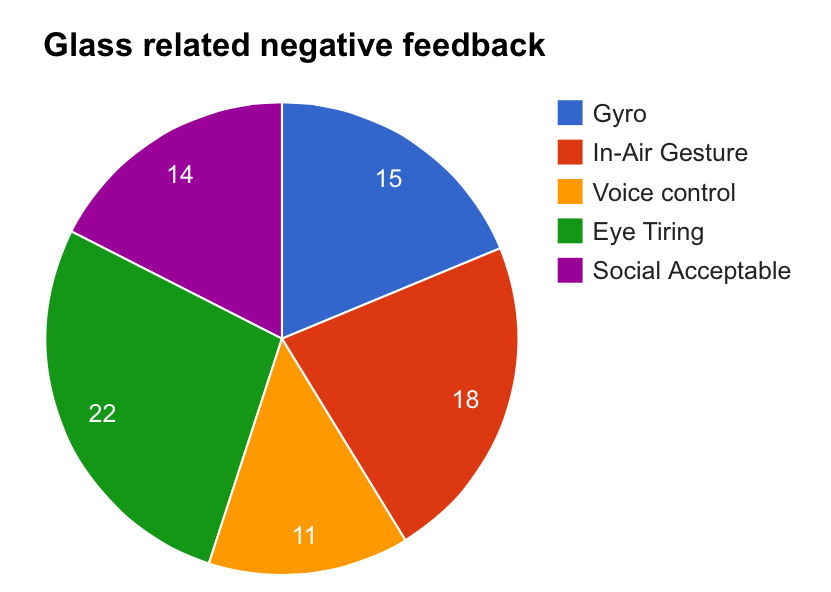
\includegraphics[width=0.9\columnwidth]{Figures/US1_userfeedbackStatistics.png}
\caption{Hi I'm Small Sun.}
\label{fig:PS_Frus}
\end{figure}


\subsection{Observation}
% \begin{enumerate}
% \item NOT social acceptable != NOT fun
% \item Small movement is better
% \end{enumerate}
From user feedback, although social acceptable would make an influence on glass game play experience, most users still think game play experience is fun and interesting. With this condition, we can conclude that social acceptable is independent to the level of fun and enjoyment. In other words, if a game has low social acceptable rate, it does not mean the game is not fun or users don't like it. In addition, we also find that small movement interacting with google glass is better and more perferred for users. 


\subsection{User imagination}
After playing all four games, we also asked users to imagine what kind of games on google glass will they like the most in user study 1. With existing glass game scene and users' originality, they brought up thirty-seven interesting glass game scenario in total. We divided them into six types of game, ``First-Person Shooter'', ``Reality Puzzle Game'', ``Social Game'', ``Sport Game'', ``Management Game'', and ``Others'' respectively (see Figure~\ref{fig:US1_TypesOfGame}). We also found that one-third of users want like first-person shooter game the most. So we decided to implement a first-person shooter game which will support multiple types of control style for users. With this design, not only users can choose which control type they like the most by their own, but we also can find out the best control style from users' feedback for first-person game on google glass and design a guideline to make better game play experience.

\begin{figure}[!t]
\centering
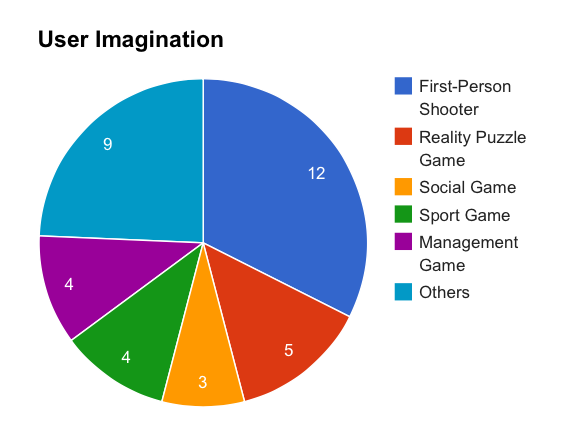
\includegraphics[width=0.9\columnwidth]{Figures/US1_userImaginationStatistics.png}
\caption{Hi I'm Small Sun 2.}
\label{fig:US1_TypesOfGame}
\end{figure}
